%% Conclusion

% general geometry reconstr + visibility info
The problem of geometry reconstruction is challenging and the diversity in scenes asks for solid solutions. The literature on geometry reconstruction is comprehensive and many approaches have been tried, with varying degrees of success. Most approaches are based on some form of photo-consistency, that is, they rely on \emph{directly} observing all objects that are being reconstructed. However, this casts constraints on the surface properties of the objects. Surfaces often need to be either uniformly coloured (low-textured) and well differentiable from the background, or they need to have clear and rich textures and Lambertian-like properties. In practice, these constraints are not always met. Therefore, many algorithms fail on certain kinds of objects.

% proposed algorithm
We proposed a new approach based on \emph{indirectly} observing objects using visibility information. Based on the intuition that detection of features from certain view points and absence of detection in others can provide clues on where occluder objects may exist, we developed two algorithms; one based on visibility information alone, and one using both visibility and occlusion (\ie absence of visibility). An occupancy grid is altered iteratively based on this information. Feature estimation is obtained by using reliable Structure from Motion tools and no pixel pair-wise guesswork needs to be done.

% results + comments / conclusion
The proposed method has been shown to provide reasonable results for scenes containing low-textured or reflective objects. For good results, enough view points need to be provided (\eg by walking around an object) and background objects containing a decent amount of features need to be present. Visibility information helps carving much of the empty space for which reliable features on background objects are extracted, but leaves space with less visibility rays partly labelled as occupied. Using both visibility and occlusion cues (and default world view `unknown') improves results, even though visibility information exported by standard structure from motion tools is often very conservative, making the majority of the occlusion claims untrue. Furthermore, the veto version of the Visibility-Occlusion algorithm (Alg. \ref{alg:vis-occ-carving-veto}) outperforms the recent dense reconstruction algorithm CMVS/PMVS on the tested reflective objects. Visibility and occlusion therefore appear promising cues for further research on geometry reconstruction. 

% future work
While sparse point clouds reconstructed by structure from motion are reliable, points do not have a clear size or shape and the exact shape of the affected space between cameras and features is therefore undefined. The taken approach of ray shooting and altering the tube of voxels hit by the ray makes the algorithm dependent on the amount of strong feature points and chosen resolution. In other words, the amount of features determines the maximum resolution. Future work could focus on relaxing those dependencies - allowing arbitrary voxel grid resolutions - by using features with better defined sizes. One possibility is to create features based on the provided sparse point cloud. For example, nearby and planar feature points can be combined to form local patches with known size and normal. They could be texture-mapped, projected into, and matched over the sequence. Potentially, small patches could also be combined using a graph-like connection map, and the changing graph over the sequence could be used for carving. The local patches could be seen as acting like small local `green screens' in the scene carving away part of space while the camera moves around.

Other features could be used as well. Edges could provide useful cues on object borders (\eg feature points disappearing after `hitting' an edge). As a last possibility, one could consider using full resolution occlusion images, for example using occlusion posterior predictions as given by the system of \Humayun2011 (for example outputs on our sequences, see Fig. \ref{fig:learningocclusions}). Hereby full-resolution probabilistic \emph{carve images} will be used instead of only a few sparse interest points. A solution needs to be found for the lack of depth, \ie where to stop carving.

Furthermore, texture mapping would make results more appealing and increases photo-realism, even for new (unseen) camera poses.

Lastly, we like to remind the reader of the observation that all current approaches - including the one proposed in this thesis - have both success stories and failure cases, but not necessarily the same failures. Therefore, the proposed approach may be used in conjunction with other approaches. For example, Visibility-Occlusion Space Carving can provide a fast and rough geometry reconstruction, which can be used as a prior for possible depths in patch-based or plane-sweeping multi-view dense reconstruction approaches.

\begin{figure}[htb!]
 \centering
 \subfigure[Frame from lampposts\_on\_wall1]{
  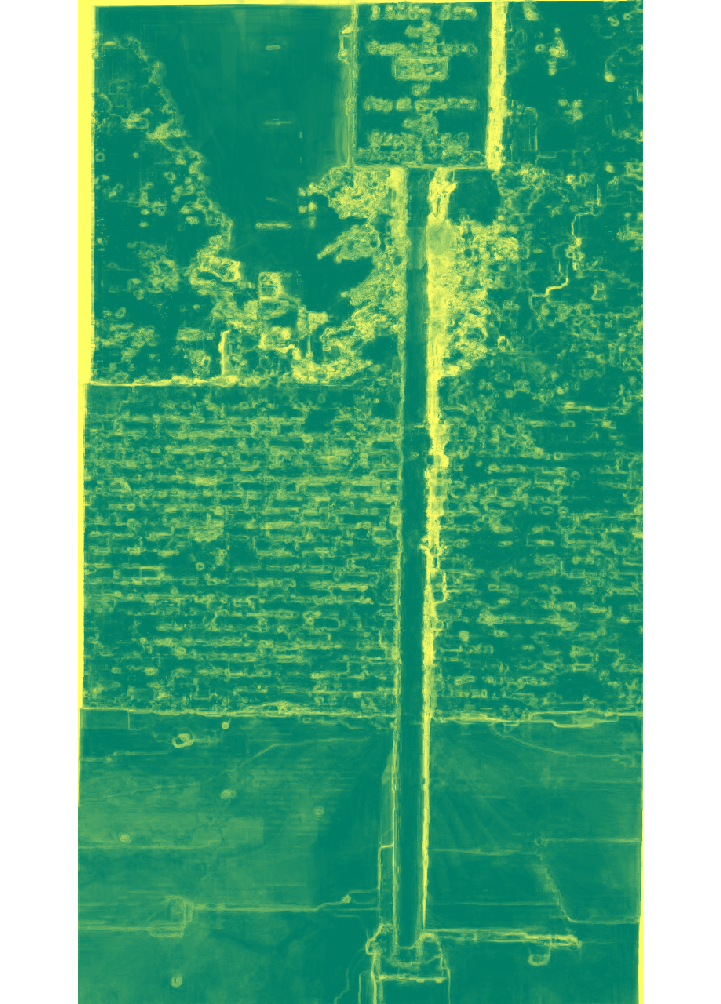
\includegraphics[width=0.35\textwidth]{img/learningocclusions1}  %\label{fig:}
 }
 \subfigure[Frame from houses1]{
  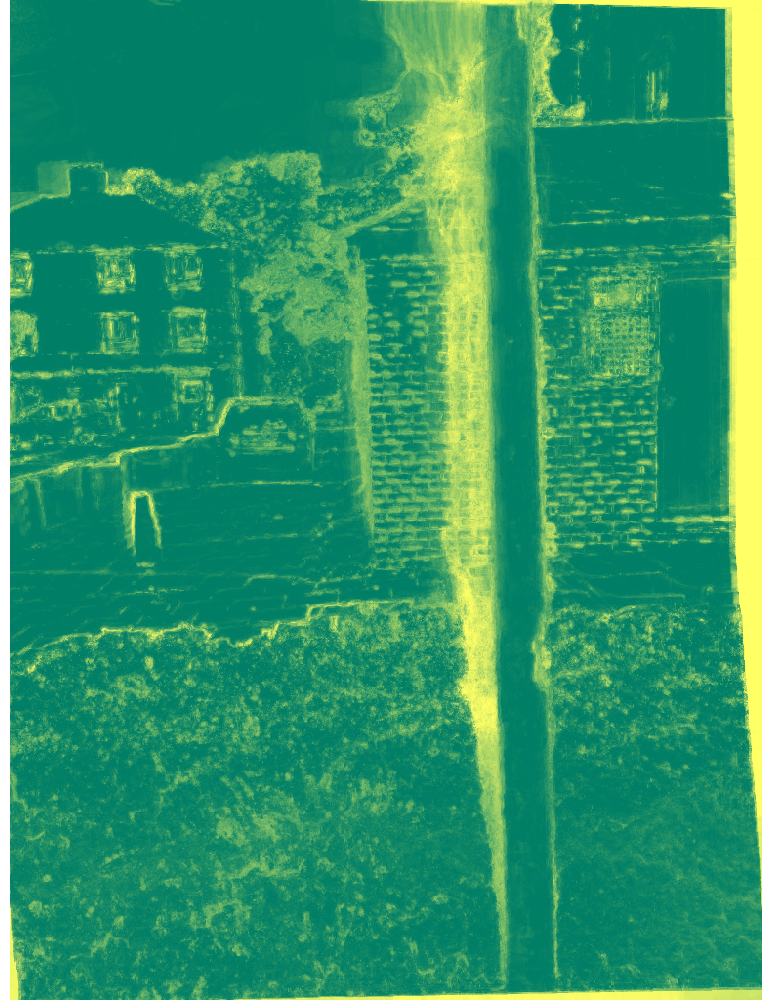
\includegraphics[width=0.35\textwidth]{img/learningocclusions2}  %\label{fig:}
 }
 \caption{Example output of the system developed by \Humayun2011, showing cyan for low and yellow for high probabilities of pixels getting occluded in the next frame}
 \label{fig:learningocclusions}
\end{figure}

